\section{The moment hierarchy and the permutation threshold}
\label{sec:theory}

\subsection{Moment conditions}
\label{sec:theory_hierarchy}

For a centred $f\in\mathcal F$ let $\gamma_j(f)=\sum_if_{ij}$ and $\rho_i(f)=\sum_jf_{ij}$ be its column and row sums; for $f=z(S)$ these are the deviations $\gamma,\rho$ of $S$.
For $\gamma\in\R^n$ put $P_\gamma(t)=\sum_{j=0}^{n-1}\gamma_jt^j$.

\begin{definition}[Degree-$k$ conditions]
\label{def:degree_k}
A centred $f\in\mathcal F$ satisfies the \emph{degree-$k$ conditions} ($k\ge1$) if $\langle x^{m},f\rangle=\langle y^{m},f\rangle=0$ for $1\le m\le k$.
For $f=z(S)$ these read $\sum_{i,j}z_{ij}x_j^m=\sum_{i,j}z_{ij}y_i^m=0$, i.e.\ $\Cov(X^m,Z)=\Cov(Y^m,Z)=0$.
\end{definition}

\begin{lemma}[Polynomial form]
\label{lem:poly_form}
If $\varphi$ depends only on the column index, $\langle\varphi,f\rangle=\frac1N\sum_j\varphi(j)\gamma_j(f)$; similarly for rows.
For $\gamma\in\R^{n}$ and $k\ge0$ the following are equivalent:
(i)~$\sum_jx_j^{m}\gamma_j=0$ for $0\le m\le k$;
(ii)~$\sum_j\binom{j}{r}\gamma_j=0$ for $0\le r\le k$;
(iii)~$(t-1)^{k+1}$ divides $P_\gamma(t)$.
Hence a centred $f$ satisfies the degree-$k$ conditions if and only if $(t-1)^{k+1}$ divides both $P_{\gamma(f)}$ and $P_{\rho(f)}$.
\end{lemma}

\begin{proof}
The first statement is $\sum_{i,j}\varphi(j)f_{ij}=\sum_j\varphi(j)\gamma_j(f)$.
The families $(x_j^{m})_{m\le k}$ and $(\binom{j}{r})_{r\le k}$ both span the restrictions to $\{0,\dots,n-1\}$ of the polynomials of degree at most $k$ in $j$, so (i)$\Leftrightarrow$(ii); and $P_\gamma(t)=\sum_{r}\bigl(\sum_j\binom jr\gamma_j\bigr)(t-1)^{r}$ is the Taylor expansion at $t=1$, so (ii)$\Leftrightarrow$(iii).
The case $m=0$ of (i) holds for every centred $f$.
\end{proof}

\begin{proposition}[Moment hierarchy]
\label{prop:hierarchy}
Let $n\ge3$ and let $f\in\mathcal F$ be centred.
\begin{enumerate}
\item[(a)] If $\gamma(f)=\rho(f)=0$, then $\langle a(X)+b(Y),f\rangle=0$ for all functions $a,b$ on $\{x_0,\dots,x_{n-1}\}$; in particular $f$ satisfies the degree-$k$ conditions for every $k$.
For $f=z(S)$ with $S$ magic, also $\langle a(X)+b(Y)+c_1\mathbf 1_{D_{\mathrm m}}+c_2\mathbf 1_{D_{\mathrm a}},z\rangle=0$.
\item[(b)] If $k\ge n-1$, the degree-$k$ conditions imply $\gamma(f)=\rho(f)=0$.
\item[(c)] If $1\le k\le n-2$, the function $f_{ij}=\frac1n(-1)^{j}\binom{k+1}{j}$ ($0\le j\le k+1$), $f_{ij}=0$ ($j>k+1$), satisfies the degree-$k$ conditions but not the degree-$(k+1)$ conditions, and $\gamma(f)\ne0$.
\end{enumerate}
\end{proposition}

\begin{proof}
(a) is the first statement of \Cref{lem:poly_form}.  (b) A nonzero polynomial of degree at most $n-1$ is not divisible by $(t-1)^{n}$.  (c) Here $\rho(f)=0$ and $P_{\gamma(f)}(t)=(1-t)^{k+1}$.
\end{proof}

Part (a) contains the vanishing of the centre of mass $\sum_cz_c(x_c,y_c)$ and of all axial moments $\sum_cz_cx_c^m$, $\sum_cz_cy_c^m$ of a semi-magic square, in the spirit of the multipole analysis of a magic cube by Rogers and Loly \cite{rogers2005multipole}.
Parts (b) and (c) are the invertibility of a Vandermonde matrix.
The mixed moments are not determined by the line sums:

\begin{remark}[Mixed moments]
\label{rem:product_inertia}
The magic square with rows $(1,6,11,16)$, $(8,15,2,9)$, $(12,3,14,5)$, $(13,10,7,4)$ has $\sum_cz_cx_cy_c=60$.
Among the $880$ magic squares of order $4$ up to $D_4$, the product of inertia $\sum_cz_cx_cy_c$ is nonzero for $824$, takes $48$ distinct absolute values between $0$ and $60$, and $\sum_cz_cx_c^2y_c$, $\sum_cz_cx_cy_c^2$ are nonzero for $623$ and $773$ of them.
For $n=3$ the mixed moment $\sum_cz_cx_cy_c$ vanishes for all eight magic squares, because $s_c+s_{-c}=10$ for centrally opposite cells, so $z$ is odd under $(x,y)\mapsto(-x,-y)$ while $xy$ is even.
\end{remark}

\begin{corollary}[Loly's invariant {\cite{loly2004invariance}}]
\label{cor:loly}
Let $I(S)=\sum_{i,j}s_{ij}(x_{j}^{2}+y_{i}^{2})$ be the moment of inertia about the centre of the masses $s_{ij}$ placed at $(x_j,y_i)$.  For every arrangement,
\begin{equation}
I(S)=N\,\Cov\bigl(Z,\,X^{2}+Y^{2}\bigr)+\frac{n^{2}(n^{4}-1)}{12}
=\sum_j x_j^{2}\gamma_j+\sum_i y_i^{2}\rho_i+\frac{n^{2}(n^{4}-1)}{12}.
\label{eq:loly_identity}
\end{equation}
Hence $I(S)=n^{2}(n^{4}-1)/12$ if and only if the single condition $\Cov(Z,X^{2}+Y^{2})=0$ holds; it is implied by the degree-$2$ conditions, hence by the semi-magic property.
\end{corollary}

\begin{proof}
Substitute $s_{ij}=z_{ij}+\frac{N+1}2$ and use \Cref{lem:variances} and \Cref{lem:poly_form}: $\frac{N+1}2\sum_{i,j}(x_j^{2}+y_i^{2})=\frac{N+1}2\cdot\frac{n^{2}(n^{2}-1)}{6}$.
\end{proof}

Loly's derivation uses the row and column sums in the same way \cite{loly2004invariance}.
The single condition is much weaker than the degree-$2$ conditions: for $n=3$, $24{,}192$ of the $9!$ arrangements have $I=60$, while $72$ (the semi-magic squares, \Cref{rem:n3_lowmode}) satisfy the degree-$2$ conditions.
The energy $\Elow$ of \eqref{eq:Elow} combines the degree-$1$ conditions with the two diagonal conditions: $\Elow=\langle x,z\rangle^2+\langle y,z\rangle^2+(\delta_{\mathrm m}^2+\delta_{\mathrm a}^2)/N^2$.

\subsection{The permutation threshold}
\label{sec:kstar}

By \Cref{prop:hierarchy}, for real-valued $f$ the degree-$k$ conditions force equal row and column sums exactly when $k\ge n-1$.
For arrangements the deviations are integers of bounded size, and the threshold drops.

\begin{definition}
\label{def:kstar}
For $n\ge3$, $k^*(n)$ is the least $k\ge1$ such that every arrangement of order $n$ satisfying the degree-$k$ conditions is semi-magic.
\end{definition}

By \Cref{prop:hierarchy}(b), $k^*(n)\le n-1$.
By \Cref{lem:poly_form}, an arrangement satisfies the degree-$k$ conditions if and only if $\gamma$ and $\rho$ lie in the lattice
\[
\Lambda_{n,k}=\{\gamma\in\Z^{n}:(t-1)^{k+1}\mid P_\gamma(t)\}=(t-1)^{k+1}\,\Z[t]_{<n-k-1},
\]
of rank $n-k-1$.
Writing $\gamma=\gamma^+-\gamma^-$ with $\gamma^\pm\ge0$, the condition $\gamma\in\Lambda_{n,k}$ says that the multisets in which $j$ occurs $\gamma^+_j$, resp.\ $\gamma^-_j$, times have equal power sums of degrees $0,\dots,k$: a Prouhet--Tarry--Escott system \cite{wright1959prouhet,borwein2002computational}.
Small vectors in $\Lambda_{n,k}$ are classical: the Prouhet--Thue--Morse vector $\bigl((-1)^{s_2(j)}\bigr)_{0\le j<2^{k+1}}$ ($s_2$ the binary digit sum) has entries $\pm1$ and lies in $\Lambda_{2^{k+1},k}$ \cite{wright1959prouhet,allouche1999ubiquitous}, and Borwein, Erd\'elyi and K\'os construct polynomials of degree $n$ with coefficients in $\{-1,0,1\}$ vanishing to order $\ge c\sqrt{n/\log n}$ at $1$ \cite[Thm.~2.7]{BEK1999}.
The question is therefore how large $k$ can be for vectors that are column-deviation vectors of arrangements.

\begin{theorem}[The permutation threshold]
\label{thm:perm_threshold}
\leavevmode
\begin{enumerate}
\item[(a)] For all $n\ge3$, $\displaystyle k^{*}(n)\le\Bigl\lfloor\sqrt{\pi e\,(n-1)\log(n^{4}/4)}\Bigr\rfloor\le 2\sqrt{\pi e}\,\sqrt{n\log n}$.
\item[(b)] $\displaystyle\liminf_{n\to\infty}\frac{k^{*}(n)}{\sqrt n}\ge\sqrt2$.
\item[(c)] $k^{*}(n)=n-1$ for $3\le n\le13$, $k^{*}(n)=n-2$ for $14\le n\le17$, and $k^{*}(n)\le n-3$ for every $n\ge18$.  The values for $14\le n\le40$ are those of \Cref{tab:kstar}.
\end{enumerate}
\end{theorem}

The constant $2\sqrt{\pi e}$ is about $5.84$.
Part (a) improves on $k^*(n)\le n-3$ only for $n\ge166$; for smaller $n$ the exact computation behind (c) is much stronger (\Cref{fig:kstar}).
Parts (c) for $n\ge14$ and the values in \Cref{tab:kstar} rest on exact computer calculations, described in \Cref{sec:kstar_exact}.

\subsection{Proof of the upper bound}
\label{sec:kstar_upper}

\begin{lemma}[Column feasibility]
\label{lem:col_feasible}
Let $\gamma$ be the column-deviation vector of an arrangement.  For every set $J$ of $p$ columns,
\begin{equation}
\Bigl|\sum_{j\in J}\gamma_j\Bigr|\le \frac{pn(N-pn)}{2}.
\label{eq:col_feasible}
\end{equation}
In particular $|\gamma_j|\le n^{2}(n-1)/2$, $\|\gamma\|_1\le N^{2}/4$ and $\|\gamma\|_2^2\le n^5(n^2-1)/12$.  The same holds for $\rho$.
\end{lemma}

\begin{proof}
The $pn$ cells of $J$ carry distinct values, whose sum is at most that of the $pn$ largest values, $pn(2N-pn+1)/2$; subtracting $pM(n)=pn(N+1)/2$ gives the upper bound, and the lower bound is symmetric.
With $p$ the number of positive $\gamma_j$, $\|\gamma\|_1=2\sum_{\gamma_j>0}\gamma_j\le pn(N-pn)\le N^2/4$.
Finally \eqref{eq:col_feasible} says that $\gamma$ is majorised by the vector with entries $n(N-(2p-1)n)/2$, $1\le p\le n$, whose squared norm is $n^5(n^2-1)/12$, and $\|\cdot\|_2^2$ is Schur-convex.
\end{proof}

\begin{lemma}[Order of vanishing of an integer polynomial at $1$]
\label{lem:jensen}
Let $\gamma\in\Z^{n}\setminus\{0\}$ with $(t-1)^{K}\mid P_\gamma$ for some $K\ge1$.  Then $K^{2}\le \pi e\,(n-1)\log\|\gamma\|_1$.
\end{lemma}

\begin{proof}
Write $P=P_\gamma$ and $L=\|\gamma\|_1$; note $K\le\deg P\le n-1$.
Since $P$ has integer coefficients and leading coefficient $a\ne0$, Jensen's formula gives
$\int_{-1/2}^{1/2}\log|P(e^{2\pi i\theta})|\,d\theta=\log\bigl(|a|\prod_\alpha\max(1,|\alpha|)\bigr)\ge0$, the product over the roots of $P$.
On $|z|=1$ we have $|P(z)|\le L$.
Since $P^{(i)}(1)=0$ for $i<K$, Taylor's formula with integral remainder along the segment $[1,z]$, which lies in the closed unit disc when $|z|=1$, gives
\[
|P(z)|\le\frac{|z-1|^{K}}{K!}\max_{|w|\le1}|P^{(K)}(w)|\le L\binom{n-1}{K}|z-1|^{K}\le L\Bigl(\frac{e(n-1)|z-1|}{K}\Bigr)^{K},
\]
because $|P^{(K)}(w)|\le\sum_j|\gamma_j|\,j(j-1)\cdots(j-K+1)$ for $|w|\le1$.
With $|e^{2\pi i\theta}-1|\le2\pi|\theta|$ and $\beta=2\pi e(n-1)/K\ge2\pi e$ we get $\log|P(e^{2\pi i\theta})|\le\log L+K\log\min(1,\beta|\theta|)$, and
$\int_{-1/2}^{1/2}\log\min(1,\beta|\theta|)\,d\theta=-2/\beta$.
Hence $0\le\log L-2K/\beta=\log L-K^{2}/(\pi e(n-1))$.
\end{proof}

\begin{proof}[Proof of \Cref{thm:perm_threshold}(a)]
Let $S$ satisfy the degree-$k$ conditions with $(k+1)^2>\pi e(n-1)\log(n^4/4)$.
If $\gamma\ne0$, then $(t-1)^{k+1}\mid P_\gamma$ (\Cref{lem:poly_form}) and $\|\gamma\|_1\le n^4/4$ (\Cref{lem:col_feasible}), contradicting \Cref{lem:jensen}.
So $\gamma=0$, and likewise $\rho=0$.
The second inequality follows from $(n-1)\log(n^4/4)<4n\log n$.
\end{proof}

The order $\sqrt{n\log n}$ also follows from \cite[Thm.~2.1]{BEK1999}, applied to $P_\gamma(t)/(t^{r}\max_j|\gamma_j|)$ with $r$ the index of the first nonzero $\gamma_j$; that theorem bounds the number of zeros at $1$ of $\sum_{j\le n}a_jt^j$ with $|a_j|\le1$ by $c\sqrt{n(1-\log|a_0|)}$, with an unspecified absolute constant.
\Cref{lem:jensen} is a self-contained version for integer coefficients.
An argument using only that $\gamma$ is a nonzero integer vector with $\|\gamma\|_\infty\le n^3$ cannot give an upper bound of smaller order than $\sqrt n$: the box principle applied to the vectors in $\{0,\dots,n^3\}^n$ and their binomial moments of order $<K$ produces such vectors in $\Lambda_{n,K-1}$ with $K\asymp\sqrt n$.

\subsection{Proof of the lower bound}
\label{sec:kstar_lower}

A lower bound $k^*(n)\ge K$ requires an arrangement that satisfies the degree-$(K-1)$ conditions without being semi-magic.
We keep all row sums equal to $M(n)$ and control the column deviations by swaps.

\begin{definition}
Rows $i\ne i'$ of an arrangement are \emph{twins on} a set $J$ of columns if $s_{ij}+s_{i'j}=N+1$ for all $j\in J$.
\end{definition}

\begin{lemma}[Twin swaps]
\label{lem:twin}
Let $S$ be semi-magic, let rows $i,i'$ be twins on $J$, let $j,j'\in J$ and $d=s_{ij'}-s_{ij}$.
Exchanging the entries of row $i$ in columns $j,j'$ changes the column deviations by $d(e_j-e_{j'})$, exchanging those of row $i'$ changes them by $-d(e_j-e_{j'})$, and neither changes a row sum.
Exchanges involving pairwise disjoint sets of cells can be combined, and their effects add.
\end{lemma}

\begin{proof}
$s_{i'j}-s_{i'j'}=(N+1-s_{ij})-(N+1-s_{ij'})=d$.
\end{proof}

\begin{lemma}[Squares with many twin rows]
\label{lem:twin_squares}
\leavevmode
\begin{enumerate}
\item If $n=2m$ with $m$ even, or with $m$ odd and $m\ge7$, there is a semi-magic square of order $n$ in which rows $r$ and $m+r$ are twins on all columns, for $0\le r<m$.
\item If $n\ge9$ is odd, there is a semi-magic square of order $n$ in which rows $\ell$ and $n-1-\ell$ are twins on the columns $\ell+1,\dots,n-2-\ell$, for $0\le\ell\le(n-9)/2$.
\end{enumerate}
\end{lemma}

The proof is a direct construction, given in \Cref{sec:app_twin}.

\begin{proposition}[Box-principle criterion]
\label{prop:box}
Let $S$ be a square of \Cref{lem:twin_squares}.
Pair the columns as $(j_q,j_q+1)$, where $j_q=2q$ for $q<Q=n/2$ ($n$ even) and $j_q=2q+1$ for $q<Q=(n-3)/2$ ($n$ odd), and let $R_q$ be the number of twin pairs of rows that are twins on both columns of the $q$-th pair: $R_q=n/2$ for even $n$, and $R_q=\min(2q,\,n-4-2q,\,(n-9)/2)+1$ for odd $n$.
If $K\ge2$ and
\begin{equation}
\prod_{q<Q}\Bigl(\Bigl\lceil\frac{R_q}2\Bigr\rceil+1\Bigr)\ >\ \prod_{r=0}^{K-2}\Bigl((N-1)\sum_{q<Q}R_q\binom qr+1\Bigr),
\label{eq:box}
\end{equation}
then there is an arrangement with all row sums $M(n)$ and $\gamma\ne0$ that satisfies the degree-$(K-1)$ conditions; hence $k^*(n)\ge K$.
\end{proposition}

\begin{proof}
For each $q$, \Cref{lem:twin} gives $R_q$ nonzero integers $d_{q,1},\dots,d_{q,R_q}$ with $|d_{q,i}|\le N-1$, one for each twin pair covering the $q$-th column pair.
At least $\lceil R_q/2\rceil$ of them have the same sign, and their partial sums, together with $0$, form a set $F_q$ of $\lceil R_q/2\rceil+1$ distinct subset sums lying in an interval of length at most $R_q(N-1)$.
For $g\in\prod_qF_q$ the integers $\mu_r(g)=\sum_qg_q\binom qr$, $0\le r\le K-2$, lie in intervals of lengths at most $(N-1)\sum_qR_q\binom qr$, so by \eqref{eq:box} there are $g\ne g'$ with $\mu_r(g)=\mu_r(g')$ for all $r\le K-2$.
Write $g_q=\sum_{i\in I_q}d_{q,i}$ and $g'_q=\sum_{i\in I'_q}d_{q,i}$.
Perform the row-$i$ exchange of \Cref{lem:twin} for the twin pairs in $I_q\setminus I'_q$ and the twin-row exchange for those in $I'_q\setminus I_q$, for every $q$; all these exchanges involve disjoint cells.
The result has all row sums $M(n)$ and $\gamma=\sum_q h_q(e_{j_q}-e_{j_q+1})$ with $h=g-g'\ne0$.
Then $P_\gamma(t)=t^{j_0}(1-t)H(t^2)$ with $H(u)=\sum_qh_qu^q\ne0$.
Since $\sum_qh_q\binom qr=0$ for $r\le K-2$, \Cref{lem:poly_form} gives $(u-1)^{K-1}\mid H(u)$, so $(t^2-1)^{K-1}\mid H(t^2)$ and $(t-1)^{K}\mid P_\gamma$.
With $\rho=0$, the arrangement satisfies the degree-$(K-1)$ conditions, and $\gamma\ne0$.
\end{proof}

\begin{proof}[Proof of \Cref{thm:perm_threshold}(b)]
Fix $\alpha<\sqrt2$ and let $K-1=k=\lfloor\alpha\sqrt n\rfloor$; we show that \eqref{eq:box} holds for all large $n$ covered by \Cref{lem:twin_squares} (every $n\ge14$ is covered).
\emph{Right side.} $\sum_{q<Q}\binom qr=\binom Q{r+1}\le\binom n{r+1}$, $R_q\le n$ and $N\le n^2$, so each factor is at most $n^4\binom n{r+1}$, and with $\log s!\ge s\log s-s$,
\[
\log(\text{right side})\le4k\log n+\sum_{s=1}^{k}\bigl(s\log n-\log s!\bigr)\le\frac{k^2}2\log\frac nk+O(k^2+k\log n)=\frac{\alpha^2}4\,n\log n+O(n).
\]
\emph{Left side.} For even $n$ it equals $(\lceil n/4\rceil+1)^{n/2}$, with logarithm $\frac n2\log n-O(n)$.
For odd $n$, $R_q\ge\min(q+1,\,Q-q,\,(n-9)/2)$, and $\min(q+1,Q-q)\le(Q+1)/2<(n-9)/2$ for large $n$, so the logarithm is at least $2\log(\lfloor Q/2\rfloor!)-O(n)=\frac n2\log n-O(n)$.
Since $\alpha^2/4<1/2$, \eqref{eq:box} holds for large $n$, and $k^*(n)\ge\lfloor\alpha\sqrt n\rfloor+1$.
\end{proof}

The convergence in (b) is slow: \eqref{eq:box} itself gives only $k^*(n)\ge2$ at $n=14$ and $k^*(n)\ge7$ at $n=100$.
Thus
\[
(\sqrt2-o(1))\sqrt n\le k^*(n)\le(2\sqrt{\pi e}+o(1))\sqrt{n\log n},
\]
and the factor $\sqrt{\log n}$ between the bounds is the analogue of the gap between $\sqrt{n/\log n}$ and $\sqrt n$ left open in \cite{BEK1999} for polynomials with coefficients in $\{-1,0,1\}$.

\subsection{Exact values}
\label{sec:kstar_exact}

\begin{proof}[Proof of \Cref{thm:perm_threshold}(c)]
\emph{$3\le n\le13$.}  Here $k^*(n)\le n-1$, and the lower bound needs an arrangement satisfying the degree-$(n-2)$ conditions that is not semi-magic.  For $n=3$ and $n=4$,
\[
\begin{pmatrix}1&3&9\\8&6&5\\7&4&2\end{pmatrix}\ \ \gamma=(1,-2,1),\ \rho=(-2,4,-2);\qquad
\begin{pmatrix}14&2&5&13\\8&15&7&4\\12&3&9&10\\1&11&16&6\end{pmatrix}\ \ \gamma=(1,-3,3,-1),\ \rho=0.
\]
In both cases $P_\gamma=(1-t)^{n-1}$ and $P_\rho\in\{0,-2(1-t)^2\}$, so the degree-$(n-2)$ conditions hold.
For $5\le n\le13$ we found arrangements with $\rho=0$ and $\gamma_j=(-1)^j\binom{n-1}j$, i.e.\ $P_\gamma=(1-t)^{n-1}$ (\Cref{sec:app_witnesses}).

\emph{$n\ge14$: level $n-2$.}  $\Lambda_{n,n-2}$ has rank $1$ and is spanned by $v=\bigl((-1)^j\binom{n-1}j\bigr)_j$.  If $\gamma=tv\ne0$ with $t\in\Z$, then $\max_j|\gamma_j|\ge\binom{n-1}{\lfloor(n-1)/2\rfloor}$, which exceeds $n^2(n-1)/2$ for $n\ge14$, contradicting \Cref{lem:col_feasible}.
(At $n=14$, $\binom{13}6=1716>1274$; passing from $n$ to $n+1$ multiplies the left side by $2$ for even $n$ and by $2n/(n+1)\ge15/8$ for odd $n\ge15$, and the right side by $(n+1)^2/(n(n-1))$, which decreases in $n$ and equals $225/182<15/8$ at $n=14$.)
So $k^*(n)\le n-2$ for $n\ge14$; at $n=13$ the bound fails ($\binom{12}6=924<1014$), and the witness has central entry $924$.

\emph{$n\ge18$: level $n-3$.}  $\Lambda_{n,n-3}$ has rank $2$: $\gamma=(t-1)^{n-2}(a+bt)$ with $a,b\in\Z$.
Two consecutive central coefficients bound $|a|,|b|$, and checking all pairs $(a,b)$ in the resulting box shows that for $18\le n\le400$ no nonzero $\gamma\in\Lambda_{n,n-3}$ satisfies $|\gamma_j|\le n^2(n-1)/2$.
For $n\ge166$, part (a) gives $k^*(n)\le n-3$, since $f(n)=(n-2)^2-\pi e(n-1)\log(n^4/4)$ is positive at $n=166$ and $f'(n)\ge2(n-2)-4\pi e(\log n+1)>0$ for $n\ge166$ (the last expression increases for $n\ge18$ and is positive at $n=166$).

\emph{Upper bounds for $14\le n\le 40$.}  If no nonzero vector of $\Lambda_{n,k}$ satisfies \eqref{eq:col_feasible} for every $p$, then $k^*(n)\le k$.  By \Cref{lem:col_feasible} it suffices to examine the vectors of $\Lambda_{n,k}$ with $\|\gamma\|_2^2\le n^5(n^2-1)/12$; we enumerated them exactly (LLL reduction followed by Fincke--Pohst enumeration in rational arithmetic, \Cref{sec:appendix}).
At the level $k=k^*(n)$ of \Cref{tab:kstar}, no nonzero vector passes the test.

\emph{Lower bounds for $14\le n\le 40$.}  For each $n$ we found an arrangement with all row sums $M(n)$ whose column deviations satisfy $(t-1)^{k^*(n)}\mid P_\gamma$ and $\gamma\ne0$; each was verified in exact integer arithmetic.
\end{proof}

\begin{table}[htbp]
\centering\footnotesize
\setlength{\tabcolsep}{2.9pt}
\begin{tabular}{r|rrrrrrrrrrrrrr}
$n$ & 14&15&16&17&18&19&20&21&22&23&24&25&26&27\\ \hline
$k^{*}(n)$ & 12&13&14&15&15&16&16&17&17&18&18&19&19&20\\
$\max_j|\gamma_j|$ & 297&572&1001&2002&1430&2860&1794&3094&2210&3638&2380&4522&2736&4541\\
$n^2(n-1)/2$ & 1274&1575&1920&2312&2754&3249&3800&4410&5082&5819&6624&7500&8450&9477\\[5pt]
$n$ & 28&29&30&31&32&33&34&35&36&37&38&39&40&\\ \hline
$k^{*}(n)$ & 21&21&22&22&23&23&23&24&24&25&25&26&26&\\
$\max_j|\gamma_j|$ & 8892&6405&11737&9330&14881&11799&9177&18147&14766&24150&16515&26520&22233&\\
$n^2(n-1)/2$ & 10584&11774&13050&14415&15872&17424&19074&20825&22680&24642&26714&28899&31200&
\end{tabular}
\caption{Exact values of the permutation threshold for $14\le n\le40$ (\Cref{thm:perm_threshold}(c)), the largest column deviation $\max_j|\gamma_j|$ of the witness arrangement, and the bound $n^2(n-1)/2$ of \Cref{lem:col_feasible}. The upper bounds come from the exact lattice enumeration of \texttt{anc/kstar\_verify.py}; for $n\le33$ they were also reproduced by an independent integer-programming computation (\texttt{anc/kstar\_crosscheck/}), so for $34\le n\le40$ they rest on the lattice enumeration alone.}
\label{tab:kstar}
\end{table}

\begin{figure}[htbp]
\centering
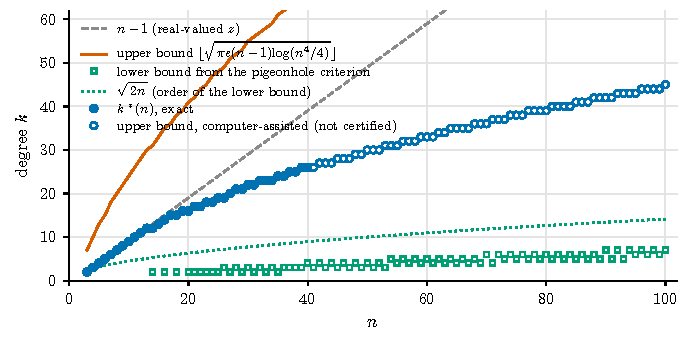
\includegraphics[width=0.72\textwidth]{figures/fig_kstar.pdf}
\caption{The permutation threshold. Exact values of $k^*(n)$ for $3\le n\le40$ (dots), the upper bounds obtained by the exact lattice enumeration for $41\le n\le100$ (open circles), the linear-algebra threshold $n-1$, the bound of \Cref{thm:perm_threshold}(a), and the curve $\sqrt{2n}$, the asymptotic order of the lower bound (b).}
\label{fig:kstar}
\end{figure}

\paragraph{The witnesses.}
The target vectors $\gamma$ were chosen among the shortest vectors of $\Lambda_{n,k^*(n)-1}$ satisfying \eqref{eq:col_feasible}, as produced by the enumeration.
Starting from a semi-magic square of \Cref{lem:twin_squares} (or a Siamese square), a steepest-descent search over exchanges within a row, which fix the row sums, minimised $\sum_j(\text{column sum}_j-M(n)-\gamma_j)^2$, with random exchanges to leave local minima; for the hardest cases a simulated annealing over arbitrary exchanges, with energy the squared distance of both row and column sums to their targets, was used.
We observe (for these $n$ only; this is not a theorem) that for $14\le n\le40$ the threshold is determined by the column-feasibility inequalities alone: $k^*(n)$ is the least $k$ for which no nonzero vector of $\Lambda_{n,k}$ satisfies \eqref{eq:col_feasible}.
Some witnesses come close to the bound of \Cref{lem:col_feasible}: $\max_j|\gamma_j|=924$ against $1014$ at $n=13$, and $24150$ against $24642$ at $n=37$.
Beyond $n=40$ we computed only upper bounds (\Cref{fig:kstar}); for instance $k^*(50)\le30$, $k^*(80)\le39$ and $k^*(100)\le45$.

\subsection{The low-order conditions for \texorpdfstring{$n=3$}{n=3}}

\begin{remark}
\label{rem:n3_lowmode}
Of the $9!$ arrangements of order $3$, exactly $760$ satisfy the degree-$1$ conditions, exactly $72$ (the semi-magic squares) satisfy the degree-$2$ conditions, and exactly $8$ satisfy the degree-$1$ conditions and both diagonal conditions, namely the magic squares (exhaustive enumeration in exact arithmetic).
So $\Elow(S)=0$ if and only if $S$ is magic when $n=3$, although the four conditions are weaker than the magic conditions for real-valued $z$.
The degree-$1$ conditions leave $\gamma=t(1,-2,1)$, $\rho=u(1,-2,1)$; the row, the column and the two diagonals through the centre cover every cell once and the centre four times, which gives $3e=15-2(t+u)$ for the centre value $e$.
We have no proof of $t=u=0$ shorter than the enumeration.
For $n=4$ the equivalence fails (\Cref{rem:four_term_insufficient}); the arrangement there has $\gamma=(3,-9,9,-3)$ and $\rho=(-6,4,10,-8)$, so it satisfies the degree-$2$ condition in $x$ but not in $y$.
\end{remark}

\subsection{Balance of the signed mass}
\label{sec:balance}

Regard $z_c$ as a signed mass at $(x_c,y_c)$.
By \Cref{prop:hierarchy}(a), a semi-magic square balances every separable test function $a(x)+b(y)$, and a magic square also the diagonal indicators; by \Cref{rem:product_inertia} it need not balance $xy$.
For arbitrary arrangements the balance is controlled by the energy:

\begin{remark}[Quantitative balance]
\label{rem:quant_balance}
Since $\sum_cz_cx_c=\sum_jx_j\gamma_j$ and $\sum_jx_j^2=n(n^2-1)/12$, the Cauchy--Schwarz inequality gives
\[
\Bigl|\sum_cz_c(x_c,y_c)\Bigr|^2\le\frac{n(n^2-1)}{12}\bigl(\|\gamma\|^2+\|\rho\|^2\bigr)\le N^2\,\frac{n(n^2-1)}{12}\,\Efull ,
\]
with equality in the first step if and only if $\gamma\parallel(x_j)$ and $\rho\parallel(y_i)$, for instance for $s_{ij}=in+j+1$.
More generally, by \Cref{lem:W_structure}, $\|P_Wz\|^2=n(\|\rho\|^2+\|\gamma\|^2)/N^2+\frac1N\delta^{\mathsf T}\Gamma_D^{-1}\delta$ with $\delta=(\delta_{\mathrm m},\delta_{\mathrm a})$, so $n\Efull\le\|P_Wz\|^2\le\lambda_n\Efull$ with $\lambda_n=n^2/(n-1)$ for odd $n$ and $n^2/(n-2)$ for even $n$; hence $|\sum_cz_c\varphi_c|\le N\|\varphi\|\sqrt{\lambda_n\Efull}$ for every $\varphi\in W$.
\end{remark}

Nonlinear balance is not implied.
With the radial unit vectors $u_c=(x_c,y_c)/|(x_c,y_c)|$ ($u_c=0$ at the centre), each of the eight $3\times3$ magic squares has $|\sum_cz_cu_c|=2(2-\sqrt2)\sqrt5\approx2.62$: for the Lo Shu with rows $(2,7,6),(9,5,1),(4,3,8)$ the edge cells contribute $(-8,4)$ and the corners $(4\sqrt2,-2\sqrt2)$.
For $n=4$ this ring imbalance is positive for all $880$ magic squares (smallest value $0.070$), with mean $5.51$ against $17.06$ for uniformly random arrangements; the magic mean lies at the $7.4$th percentile of the random distribution (\texttt{anc/balance\_check.py}).
